\documentclass{article}
\usepackage{graphicx} % For including images
\usepackage{titling}  % For custom title page
\usepackage{circuitikz}
\usepackage{amsmath}
\usepackage{amssymb}
\usepackage{booktabs,tabu}

\newcommand{\ohm}{\Omega}
% Set up title and author
\title{Experiment 1: Basic Filter Design}
\author{Samyak Sheersh, Aryam Shankar}
\date{06 August 2024}
\newcommand{\subtitle}[1]{%
  \posttitle{%
    \par\end{center}
    \begin{center}\large#1\end{center}
    \vskip0.5em}%
}

\begin{document}

% Custom title page
\begin{titlepage}
    \centering
    
\includegraphics[width=0.2\textwidth]{KGP_logo.png}\par\vspace{1cm}
    {\scshape\LARGE Department of Electronics and Electrical Communication Engineering, IIT Kharagpur\par}
    \vspace{1cm}
    {\huge\bfseries Experiment 1: Basic Filter Design\par}
    \vspace{1.5cm}
    {\Large\itshape Samyak Sheersh, Aryam Shankar\par}
    \vfill
    % Identifying information at the bottom
    {\large Roll Numbers: 22EC30045, 22EC3FP37\par}
    {\large Group Number: 12\par}
    \vfill
    {\large 06 August 2024\par}
\end{titlepage}

% Start the content of the report
\section{Introduction}
We can design a low pass filter, a high pass filter, a band pass filter using passive components, namely, a resistor and a capacitor. However since these are passive component, the signals filtered will be attenuated and won't be amplified. We calculate the threshold when the power in the signal has attenuated by half or about 3dB. 

We can design an active first order filter which amplifies the signal using an op-amp.

In the third task, we will add two signals using an op-amp.

\section{Objectives}

\emph{Note: G=12 $\Rightarrow$ (G-1) mod\ 4 = 3}

\subsection{Task 1}
\emph{Design a 1\textsuperscript{st} order passive filter with following corner frequencies:}
  \begin{enumerate}
    \item Low pass filter with cut-off frequency of $f_H = 4{(G-1) mod\ 4} +12 = 24$KHz
    \item High pass filter with cut-off frequency of $f_L = 4{(G-1) mod\ 4} +4 = 16$KHz
    \item Band pass filter with cut-off frequencies of $f_L= 16$KHz and $f_H = 24$KHz
    \item Find out the 3dB frequency from both time and frequency domain representation of signal on Digital Signal Oscilloscope
    \item Find out the amplitude of signal at $\frac{f_L}{2}, 2f_H$
  \end{enumerate}

\subsection{Task 2}
  \emph{Implement a 1\textsuperscript{st} order active low-pass filter using an op-amp with the above specifications and gain of 2. Observe the output on the DSO.}

\subsection{Task 3}
\emph{Take two voltage signals $x_1(t)$ and $x_2(t)$ and add them using Op-
Amp withfollowing formula:}
$$
y(t) = (-1)^{G}\{x_1(t) + ((G-1) mod\ 4 )x_2(t)\} = x_1(t)+3x_2(t)
$$

\section{Instruments and Materials required}
\begin{itemize}
  \item RIGOL Signal Generator
  \item ScientiFIC SMO10C Digital Signal Oscilloscope
  \item +12V, -12V DC source and ground
  \item Resistors
  \item Capacitors
  \item Breadboard
  \item Connecting wires
\end{itemize}

\section{Theory}
A low-pass filter lets a signal below a certain frequency $f_H$ pass. For a first order passive filter, we define $f_H$ to be the point at which the power of the signal gets attenuated by 3dB from the maximum power.

In a passive filter with a resistor R and capacitor C, the $f_H$ is:
$$f_H = \frac{1}{2\pi RC}$$

\vspace{2mm}
A high-pass filter lets a signal above a certain frequency $f_L$ pass. For a first order passive filter, we define $f_L$ to be the point at which the power of the signal gets attenuated by 3dB from the maximum power.

In a passive filter with a resistor R and capacitor C, the $f_H$ is:
$$f_L = \frac{1}{2\pi RC}$$

For an active low pass filter using an op-amp, the gain is:
$$Gain = \Big(1+\frac{R_f}{R_2}\Big)$$

and the $f_H$ is:
$$f_L = \frac{1}{2\pi RC}$$

\section{Calculations and Circuit Design}

\subsection{Task 1}
\subsubsection{Task 1.1}
The closest we could get to $f_H=24kHz$ was using $R=1.2k\ohm$ and $C=5.6nF$ to get $f_H=23.683kHz$

The circuit is shown below
 \begin{figure}[!ht]
        \caption{Required diagram for Task 1.1}
        \begin{center}
          \begin{circuitikz}
            \draw (2,11.25) to[sinusoidal voltage source, sources/symbol/rotate=auto,l={ $V_{in}$}] (2,8.75);
            \draw (2,11.25) to[R,l={ $R=1.2 k\ohm$}] (6.25,11.25);
            \draw (6.25,11.25) to[C,l={ $C=5.6 nF$}] (6.25,8.75);
            \draw (2,8.75) to[short] (8.5,8.75);
            \draw (6.25,11.25) to[short] (7,11.25);
            \draw (7,11.25) to[short] (8.75,11.25);
            \draw (8.5,8.75) to[short] (8.75,8.75);
            \node at (9.25,10.25) {$V_{out}$};
            \draw (6.25,11.25) to[short, -o] (8.75,11.25) ;
            \draw (7.5,8.75) to[short, -o] (8.75,8.75) ;
          \end{circuitikz}
        \end{center}
        \label{fig:lpf}
      \end{figure}
\newpage
\subsubsection{Task 1.2}

The closest we could get to $f_L=16kHz$ was using $R=1.8k\ohm$ and $C=5.6nF$ to get $f_H=15.789kHz$

   \begin{figure}[!ht]
        \caption{Required diagram for Task 1.2}
        \begin{center}
          \begin{circuitikz}
            \draw (2,11.25) to[sinusoidal voltage source, sources/symbol/rotate=auto,l={ \LARGE $V_{in}$}] (2,8.75);
            \draw (2,8.75) to[short] (8.5,8.75);
            \draw (6.25,11.25) to[short] (7,11.25);
            \draw (7,11.25) to[short] (8.75,11.25);
            \draw (8.5,8.75) to[short] (8.75,8.75);
            \node at (9.25,10.25) {$V_{out}$};
            \draw (6.25,11.25) to[short, -o] (8.75,11.25) ;
            \draw (7.5,8.75) to[short, -o] (8.75,8.75) ;
            \draw (2,11.25) to[C,l={ $C=5.6nF$}] (6.25,11.25);
            \draw (5.75,11.25) to[R,l={ $R=1.8k\ohm$}] (5.75,8.75);       
          \end{circuitikz}
        \end{center}
        \label{fig:hpf}
      \end{figure}

\subsection{Task 2}
Since the gain required is 2:
$$
\Rightarrow 1+\frac{R_f}{R_2}=2 \Rightarrow R_f=R_2
$$
We use the same LPF as before ($f_H=24KHz$), and $R_f=R_2=1k\ohm$ in the circuit.
 \begin{figure}[!ht]
    \caption{Required diagram for Task 2}
    \begin{center}
      \begin{circuitikz}
        \draw (2,12) to[R,l={ $R_1 = 1.2k\ohm$}] (5.5,12);
        \draw (5.5,12) to[C,l={$C=5.6nF$}] (5.5,6.25);
        \node at (1.5,12.25) {$V_{in}$};
        \draw (8.5,11.5) node[op amp, noinv input up] (opamp2) {};
        \draw (opamp2.+) to[short] (7,12);
        \draw  (opamp2.-) to[short] (6.75,11);
        \draw (9.7,11.5) to[short](10,11.5);
        \draw (5.5,12) to[short] (7,12);
        \draw (5.5,6.5) to (5.5,6.25) node[ground]{};
        \node at (5.5,12) [circ] {};
        \draw (9.75,11.5) to[short] (13.5,11.5);
        \node at (6.75,7.75) [circ] {};
        \draw (6.75,11) to[short] (6.75,7.75);
        \draw (6.75,7.75) to[R,l={$R_2=1k\ohm$}] (6.75,6.25);
        \draw (6.75,6.25) to[short] (5.5,6.25);
        \node at (5.5,6.25) [circ] {};
        \draw (6.75,7.75) to[short] (10,7.75);
        \draw (9.75,7.75) to[R,l={$R_f= 1k\ohm$}] (12,7.75);
        \draw (12,7.75) to[short] (12,11.5);
        \node at (12,11.5) [circ] {};
        \node at (13.75,11.75) {$V_{out}$};
        \draw (9.7,11.5) to[short](10,11.5);
      \end{circuitikz}
    \end{center}
    \label{fig:opamp-task-2}
  \end{figure}
\newpage

\subsection{Task 3}
Seeing the $R_f, R_3$ configuration as a voltage divider, we equalise the voltage in the inverting and non-inverting input at $V_i=\frac{V_{out}R_3}{R_3+R_f}$. 

Also, since the input resistance is infinite, there is no current in the input.
$$
\Rightarrow \frac{x1-V_i}{R_2}+\frac{x2-V_i}{R_1}=0 
$$
$$
\Rightarrow R_1 x_1 + R_2 x_2 = (R_1+R_2)V_i = \frac{(R_1+R_2)R_3}{R_3+R_f} V_{out}
$$

But since it's required that $V_{out} = x_1+3x_2$, we can solve the system as:
$$
R_1=1k\ohm ; R_2=3k\ohm ; R_3=1k\ohm ; R_f=3k\ohm
$$
\begin{figure}[!ht]
  \begin{center}
    \caption{Required diagram for Task 3}
    \begin{circuitikz}
      \draw (1.75,13.25) to[R,l={ \normalsize $R_2=3k\ohm$}] (5.25,13.25);
      \draw (1.75,12) to[R,l={ \normalsize $R_1=1k\ohm$}] (5.25,12);
      \draw (5.25,13.25) to[short] (5.25,12);
      \draw (6.75,12.25) node[op amp,scale=1, yscale=-1 ] (opamp2) {};
      \draw (opamp2.+) to[short] (5.25,12.75);
      \draw  (opamp2.-) to[short] (5.25,11.75);
      \draw (7.95,12.25) to[short](8.25,12.25);
      \draw (5.25,11.75) to[short] (5.25,9.75);
      \draw (5.25,9.75) to[R,l={ \normalsize $R_3=1k\ohm$}] (5.25,7.75);
      \draw (5.25,7.75) to (5.25,7.5) node[ground]{};
      \draw (8,12.25) to[short] (11.75,12.25);
      \draw (9.5,12.25) to[short] (9.5,10.25);
      \draw (9.5,10.25) to[R,l={ \normalsize $R_f=3k\ohm$}] (5.25,10.25);
      \node at (5.25,10.25) [circ] {};
      \node at (5.25,12.75) [circ] {};
      \draw (5.25,7.75) to (5.25,7.5) node[ground]{};
      \draw (11.25,12.25) to[short, -o] (11.75,12.25) ;
      \node at (9.5,12.25) [circ] {};
      \node [font=\normalsize] at (1,13.5) {$x_1(t)$};
      \node [font=\normalsize] at (1,12) {$x_2(t)$};
      \node [font=\normalsize] at (12.25,12.5) {$V_{out}$};
    \end{circuitikz}
  \end{center}
  \label{fig:opamp-task-3}
\end{figure}
\newpage
\section{Observation Tables and Figures}
\subsection{Task 1}
\subsubsection{Task 1.1}
\begin{figure}[!ht]
  \caption{Frequency response graph for Low-pass filter}
  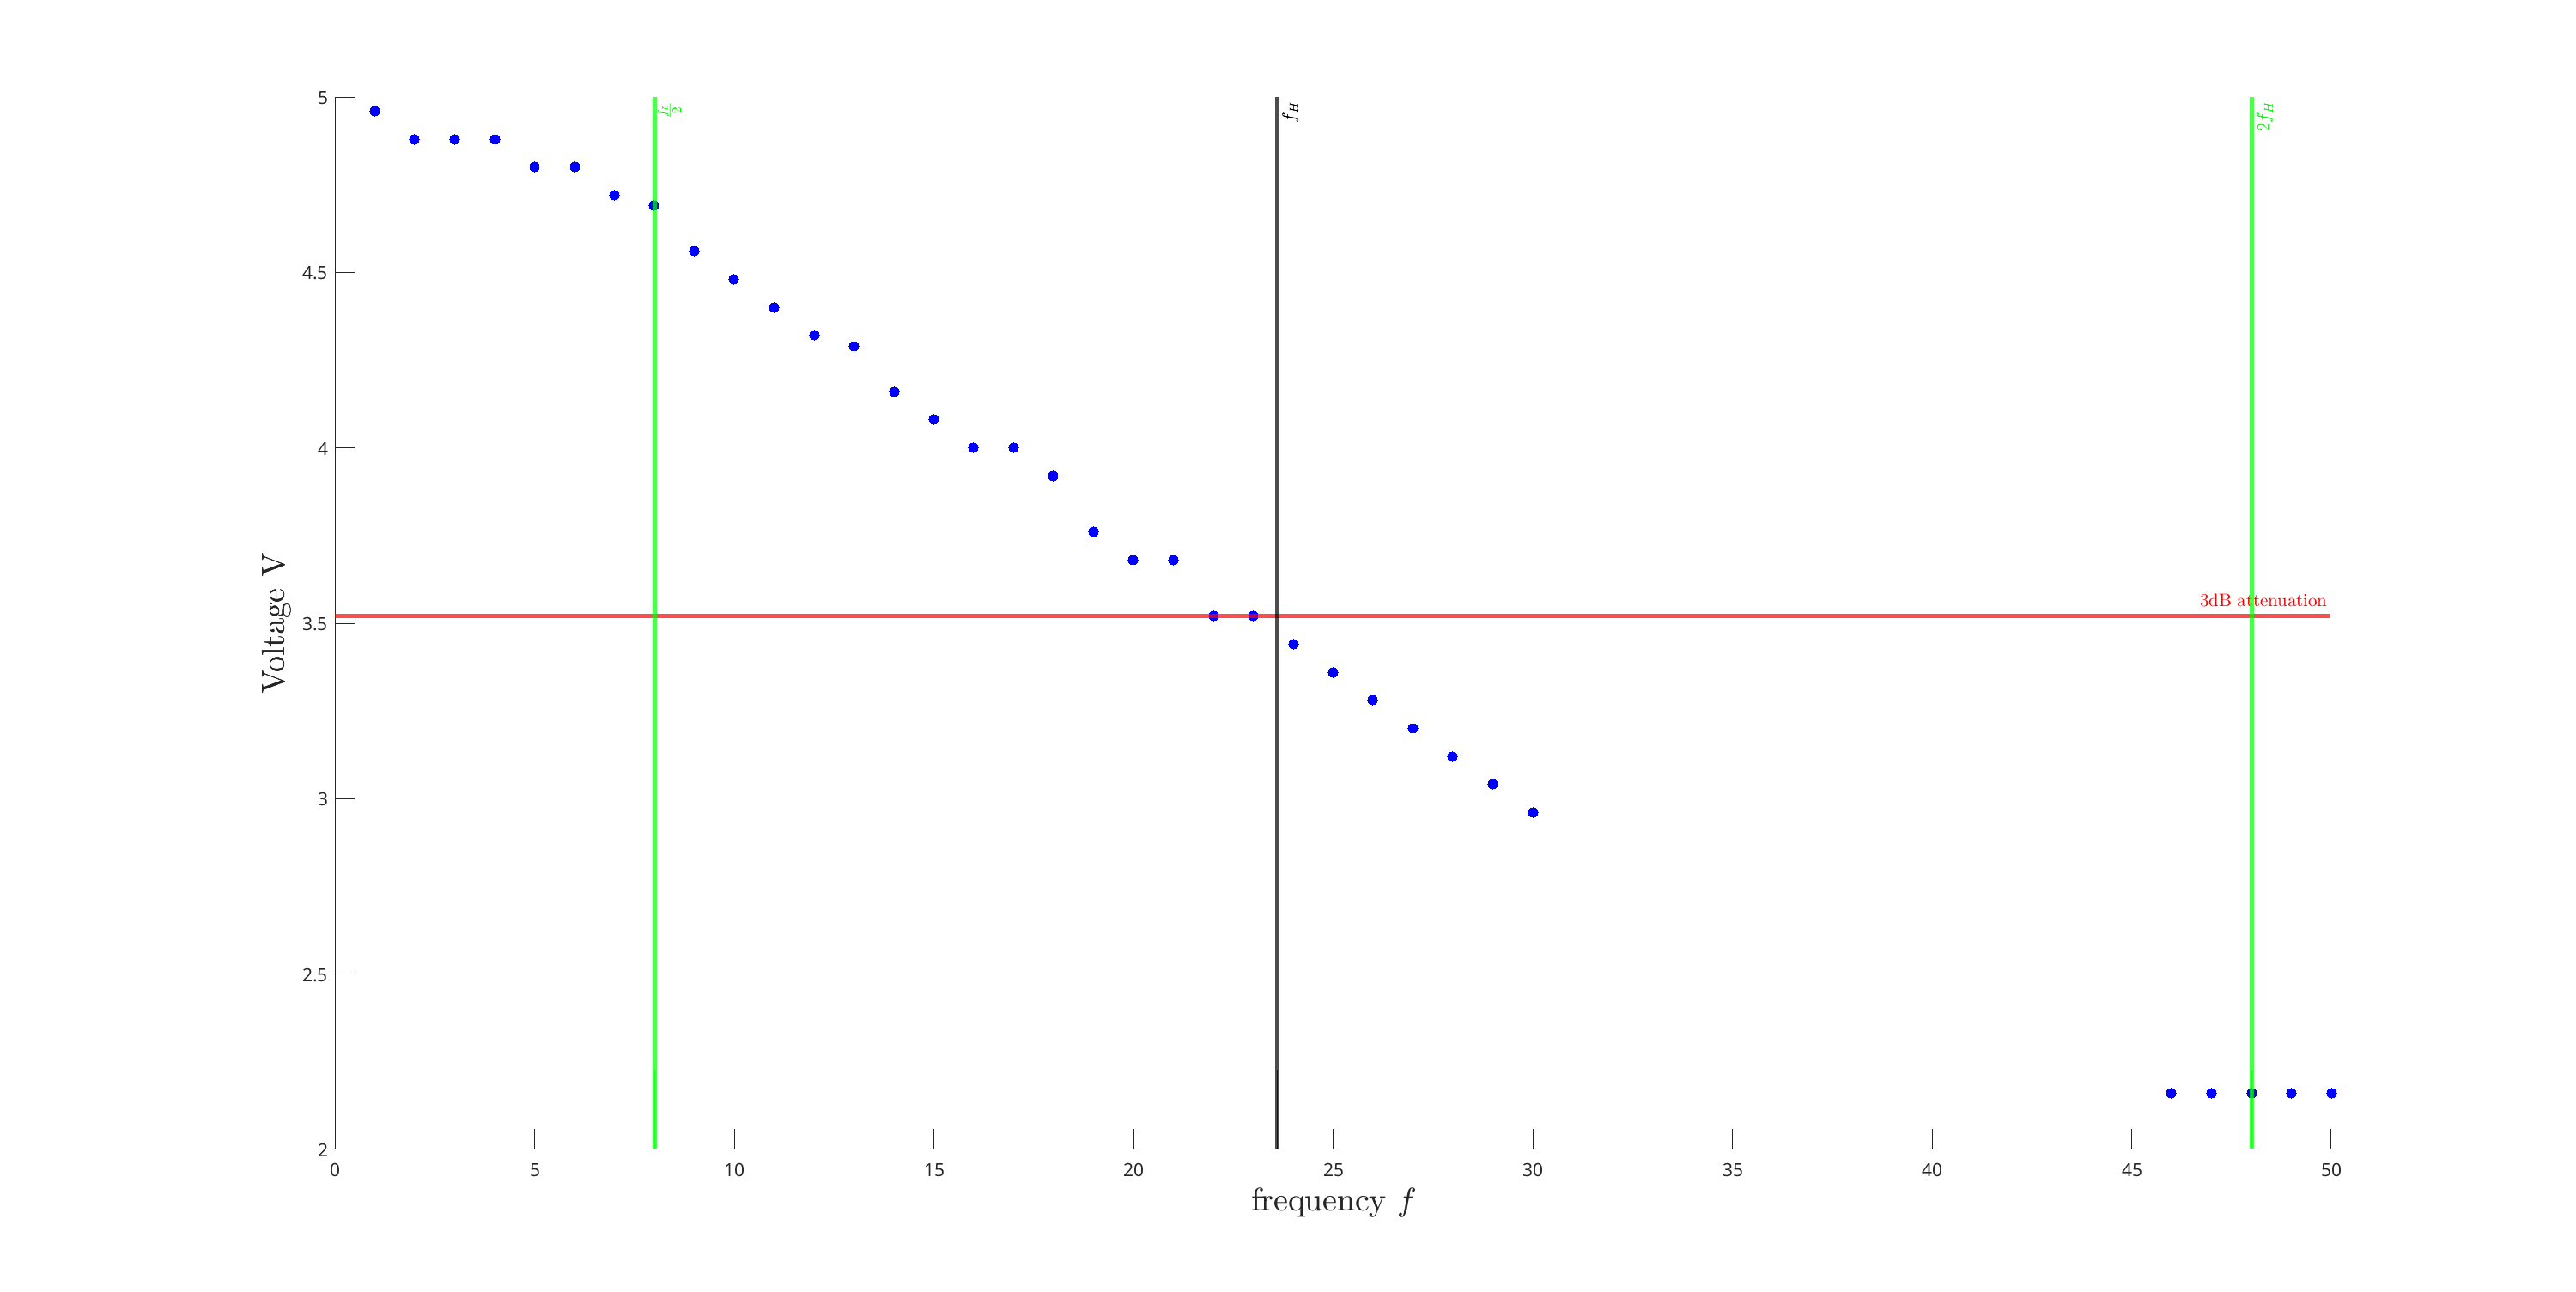
\includegraphics[width=\textwidth]{LPF.png}
  \label{fig:task-1-1}
\end{figure}

\begin{table}[!ht]
  \centering
  \caption{Frequency response observation table for Low-pass filter}
  \begin{tabu}{[2]{ll}}
    \toprule
    \textbf{Signal frequency (kHz)} & \textbf{Output Voltage(V)} \\
    \midrule
    1  & 4.96 \\ 
    2  & 4.88 \\
    3  & 4.88 \\ 
    4  & 4.88 \\ 
    5  & 4.80 \\ 
    6  & 4.80 \\ 
    7  & 4.72 \\ 
    8  & 4.69 \\ 
    9  & 4.56 \\ 
    10 & 4.48 \\ 
    11 & 4.40 \\ 
    12 & 4.32 \\ 
    13 & 4.29 \\ 
    14 & 4.16 \\ 
    15 & 4.08 \\ 
    16 & 4.00 \\ 
    17 & 4.00 \\ 
    18 & 3.92 \\ 
    19 & 3.76 \\ 
    20 & 3.68 \\ 
    21 & 3.68 \\ 
    22 & 3.52 \\ 
    23 & 3.52 \\ 
    24 & 3.44 \\ 
    25 & 3.36 \\ 
    26 & 3.28 \\ 
    27 & 3.20 \\ 
    28 & 3.12 \\ 
    29 & 3.04 \\ 
    30 & 2.96 \\ 
    46 & 2.16 \\ 
    47 & 2.16 \\ 
    48 & 2.16 \\ 
    49 & 2.16 \\ 
    50 & 2.16 \\
    \bottomrule
  \end{tabu}
  \label{tab:lpf}
\end{table}

\textbf{Results:}
\begin{enumerate}
  \item The 3dB frequency is 23KHz(The voltage decreases by $\sqrt2$, and the power by $2\approx 3dB$)
  \item The amplitude at $\frac{f_L}{2}=8kHz$ is 4.56V
  \item The amplitude at $2f_H=48kHz$ is 2.16V
\end{enumerate}
\subsubsection{Task 1.2}
\begin{figure}[!ht]
  \caption{Frequency response graph for High-pass filter}
  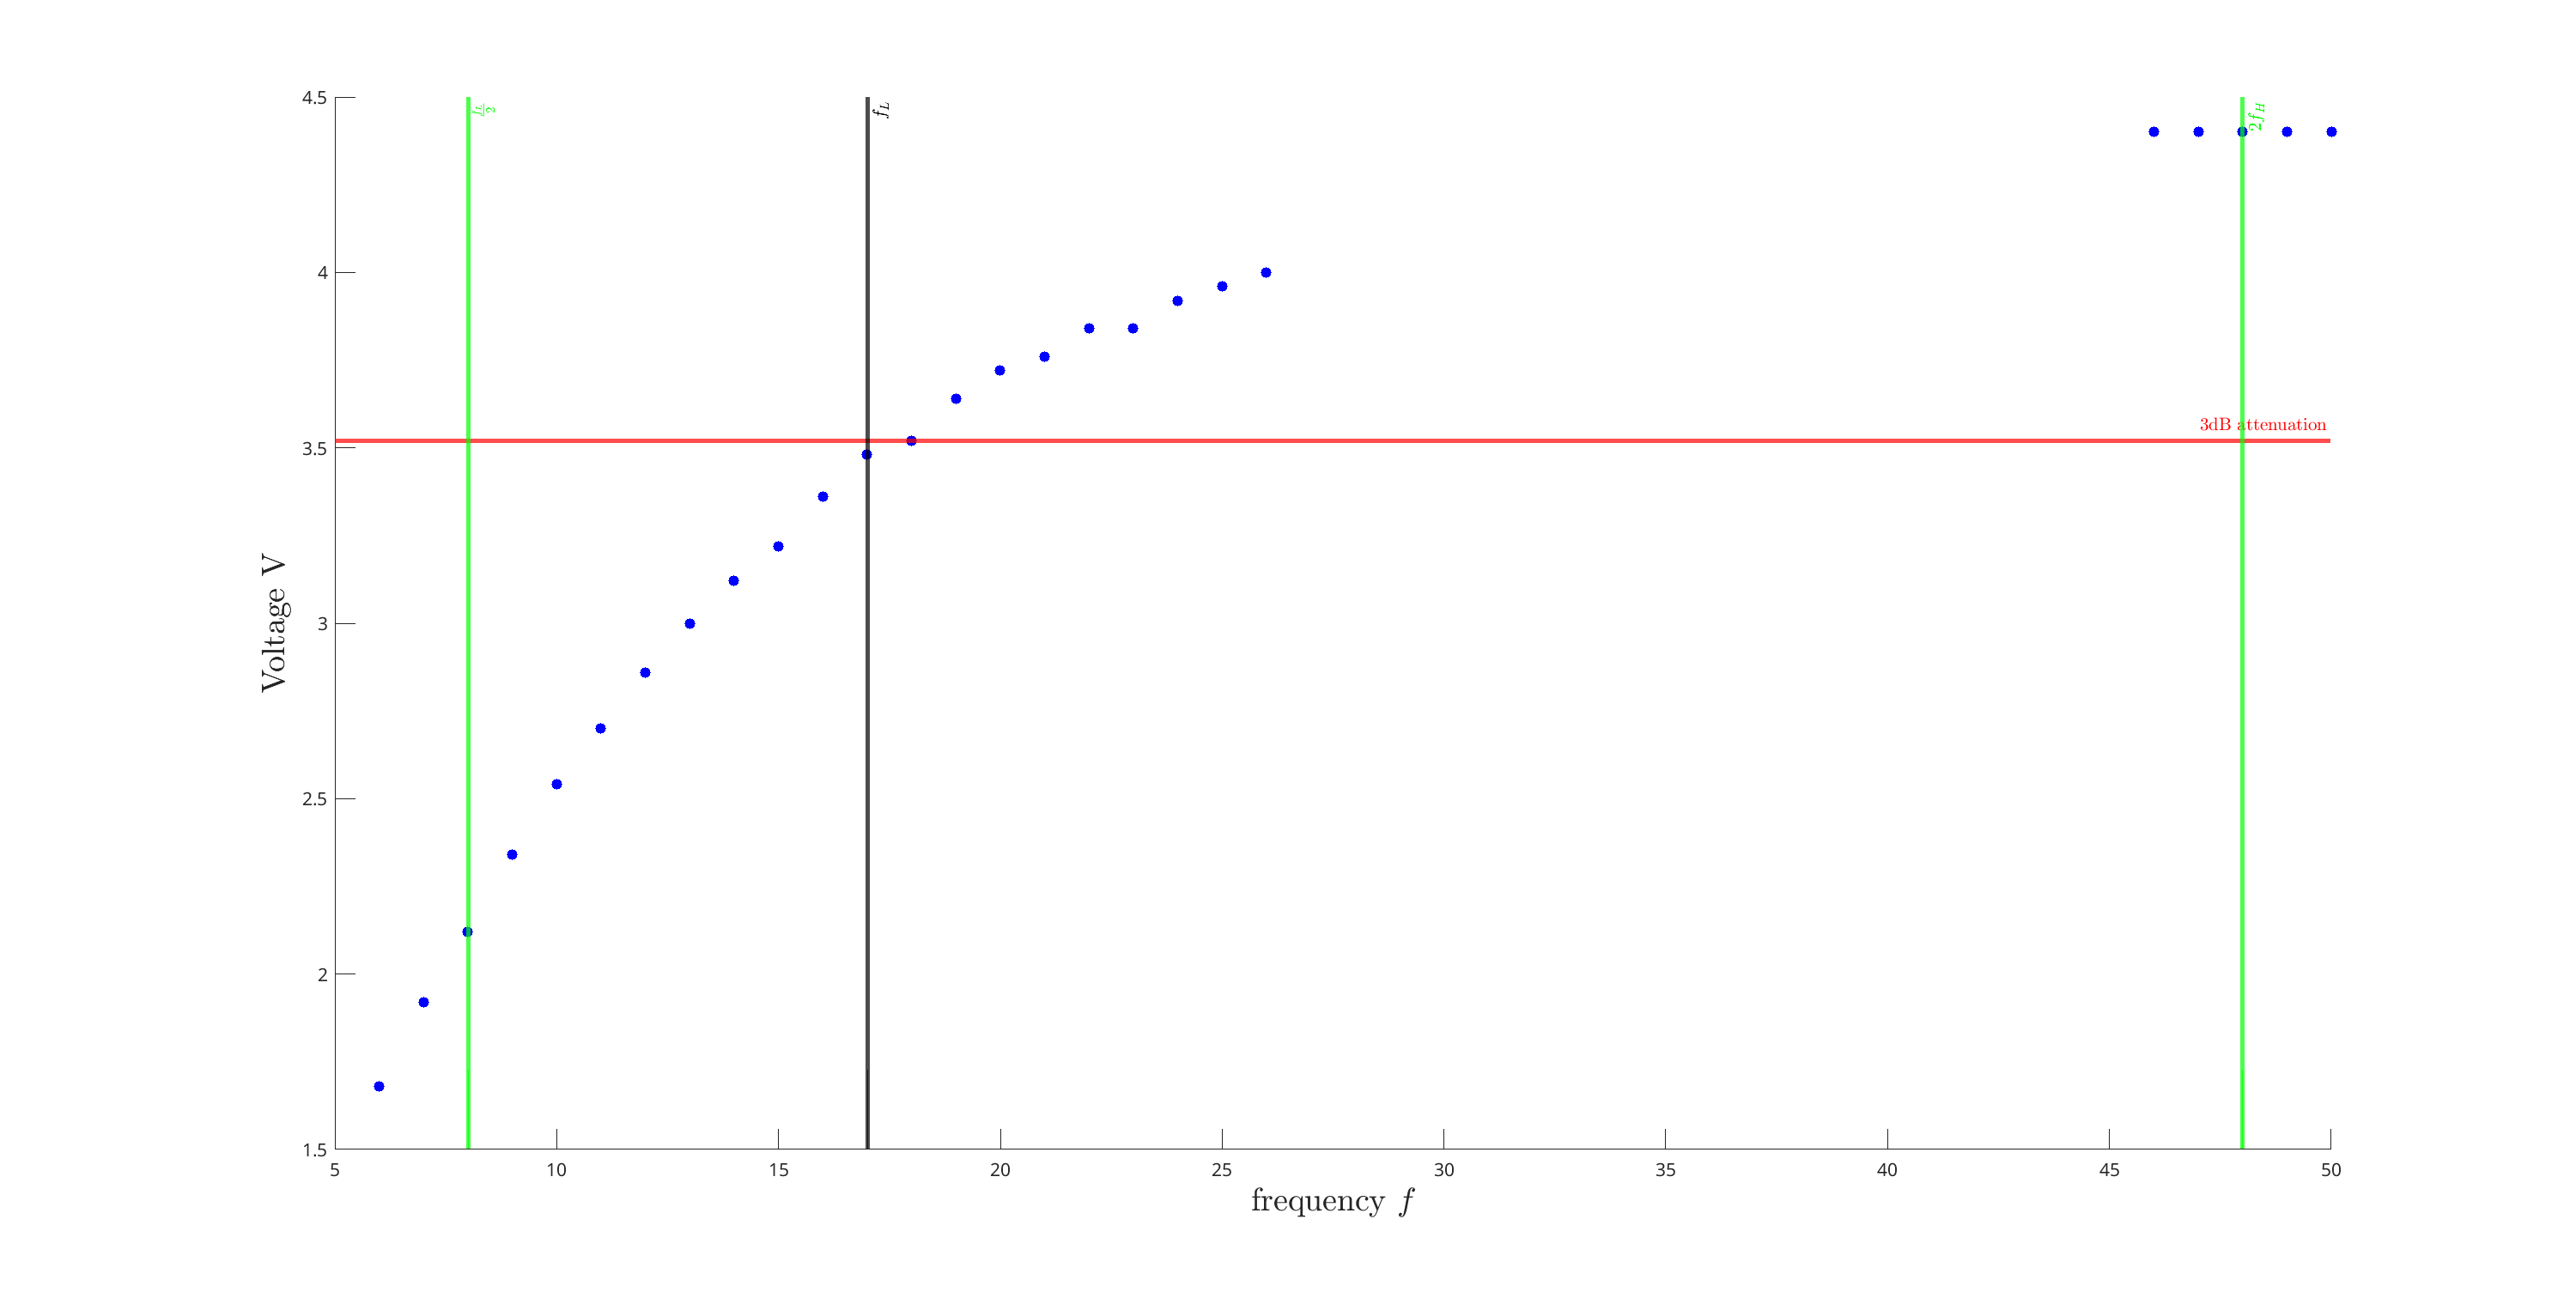
\includegraphics[width=\textwidth]{HPF.png}
  \label{fig:task-1-2}
\end{figure}

\begin{table}[!ht]
  \centering
  \caption{Frequency response observation table for High-pass filter}
  \begin{tabu}{*[2]{x[c]}}
    \toprule
    \textbf{Signal frequency (kHz)} & \textbf{Output Voltage(V)} \\
    \midrule
      6  & 1.68 \\
      7  & 1.92 \\
      8  & 2.12 \\
      9  & 2.34 \\
      10 & 2.54 \\
      11 & 2.70 \\
      12 & 2.86 \\
      13 & 3.00 \\
      14 & 3.12 \\
      15 & 3.22 \\
      16 & 3.36 \\
      17 & 3.48 \\
      18 & 3.52 \\
      19 & 3.64 \\
      20 & 3.72 \\
      21 & 3.76 \\
      22 & 3.84 \\
      23 & 3.84 \\
      24 & 3.92 \\
      25 & 3.96 \\
      26 & 4.00 \\
      46 & 4.40 \\
      47 & 4.40 \\
      48 & 4.40 \\
      49 & 4.40 \\
      50 & 4.40\\
      \bottomrule

    \end{tabu}
\end{table}
\textbf{Results:}
\begin{enumerate}
  \item The 3dB frequency is 17KHz(The voltage decreases by $\sqrt2$, and the power by $2\approx 3dB$)
  \item The amplitude at $\frac{f_L}{2}=8kHz$ is 2.12V
  \item The amplitude at $2f_H=48kHz$ is 4.40V
\end{enumerate}
\newpage

\subsubsection{Task 1.3}
\begin{figure}[!ht]
  \caption{Frequency response graph for Band-pass filter}
  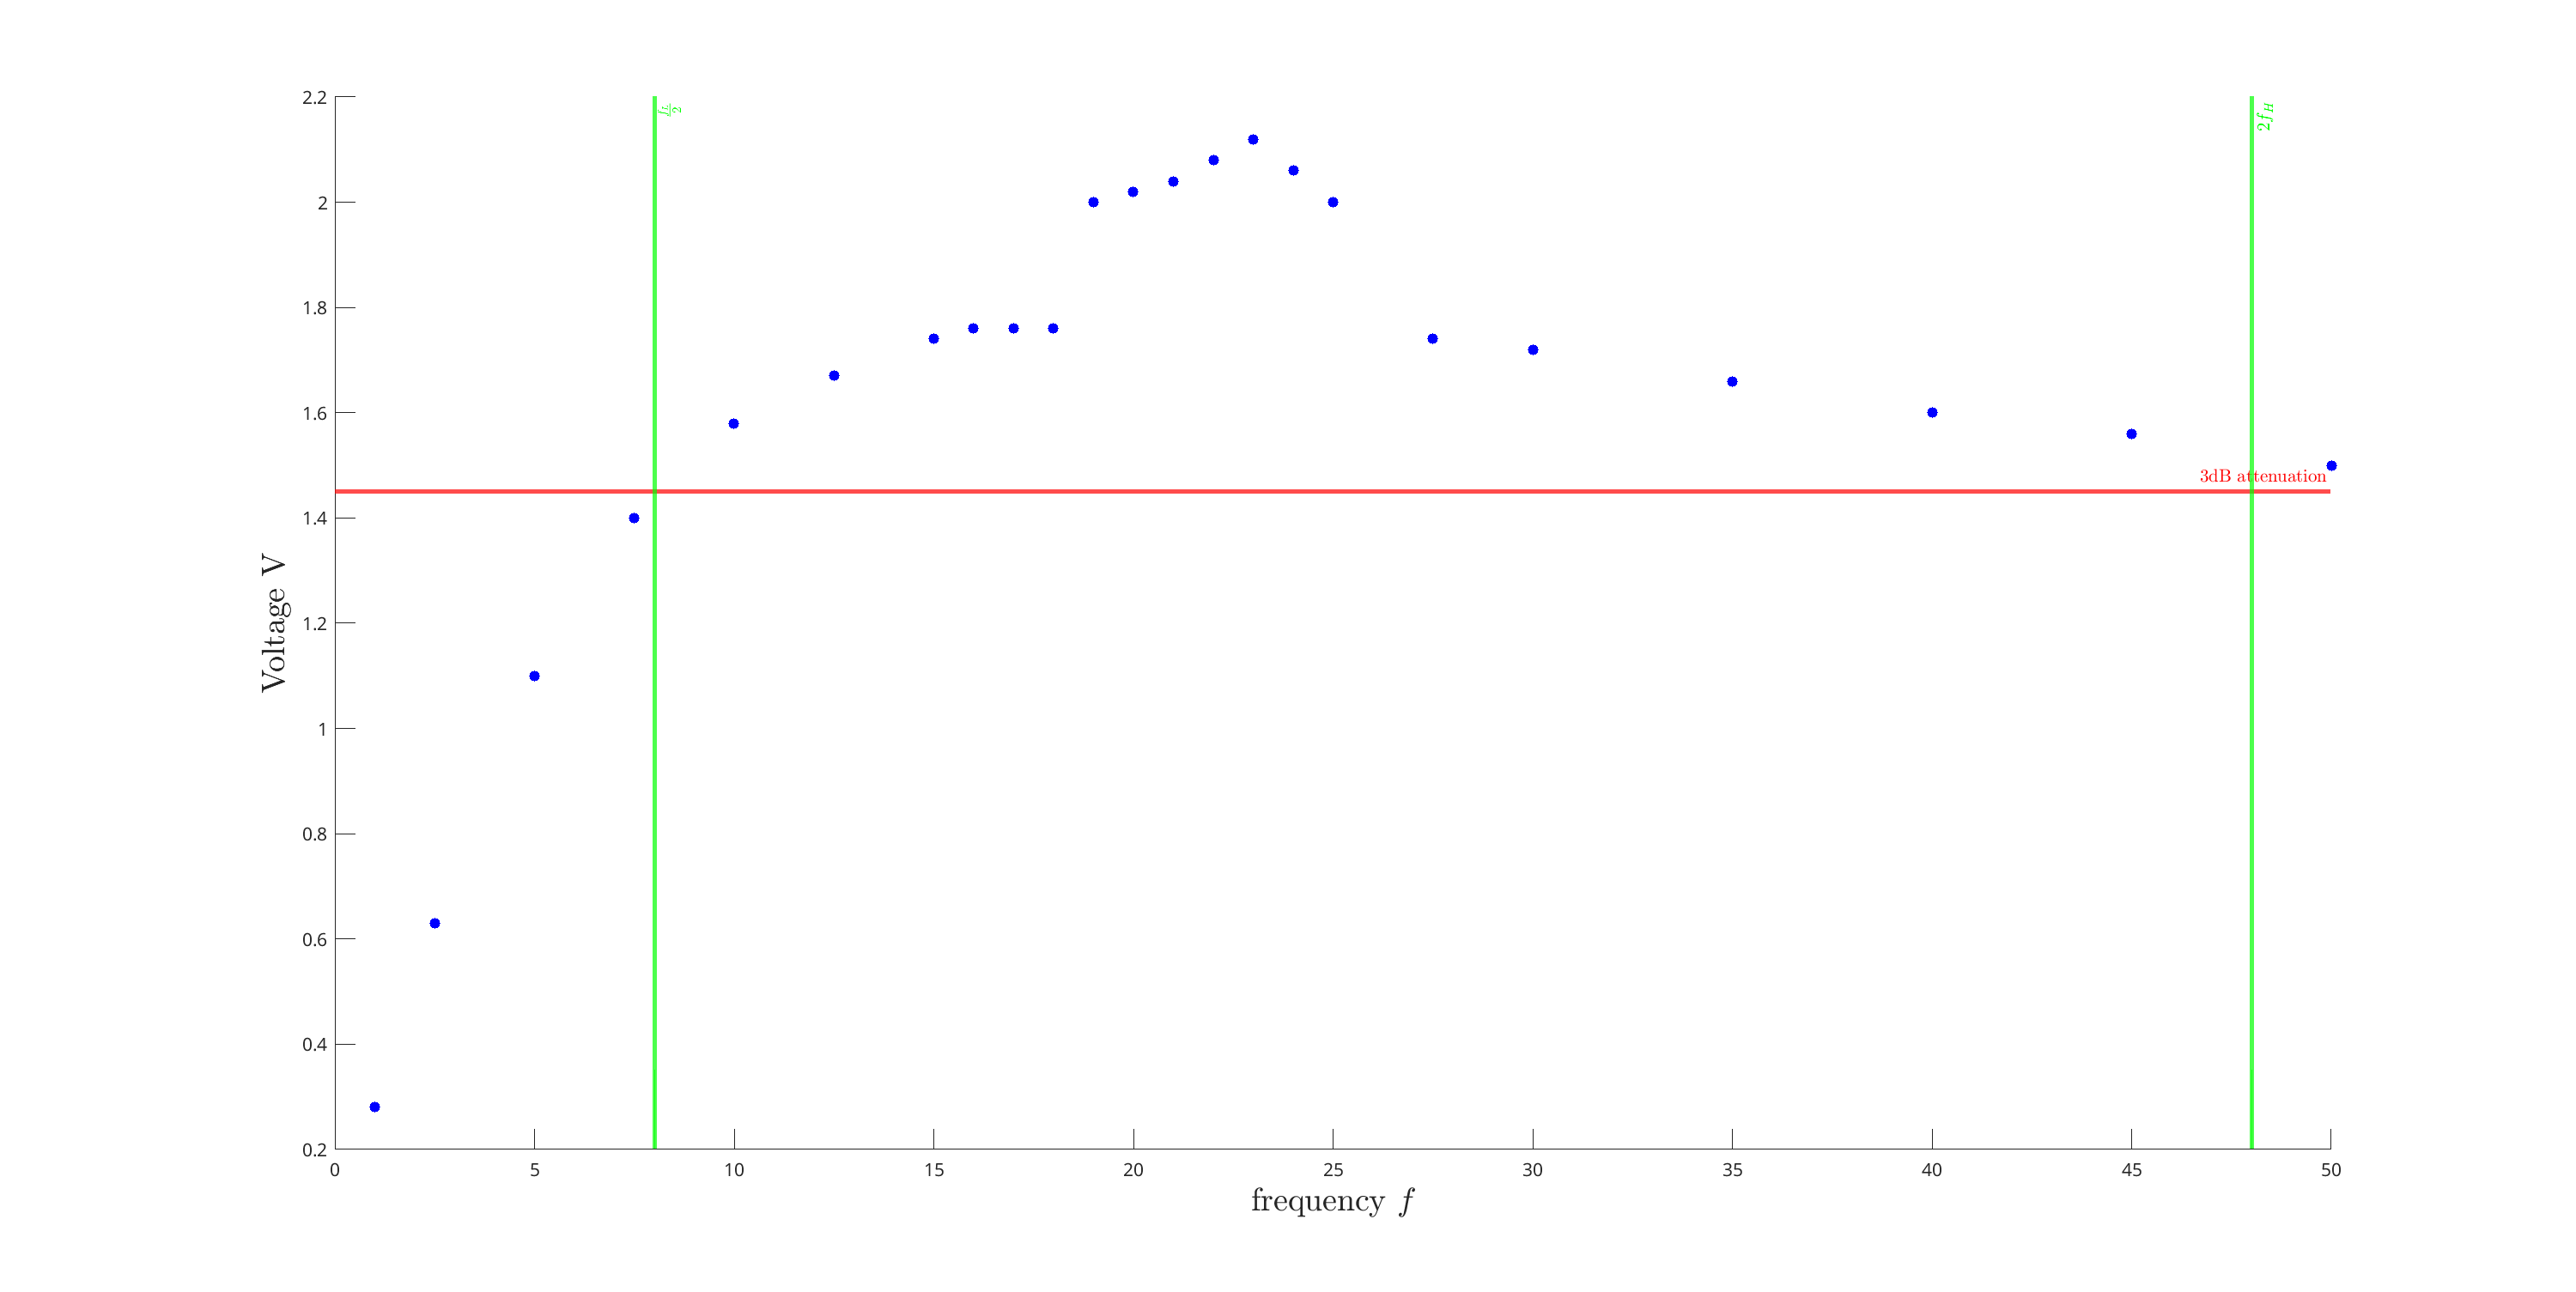
\includegraphics[width=\textwidth]{BPF.png}
  \label{fig:task-2}
\end{figure}
\begin{table}[!ht]
  \centering
  \begin{tabu}{*[2]{x[c]}}
    \toprule
    \textbf{Signal frequency (kHz)} & \textbf{Output Voltage(V)} \\
    \midrule
    4  & 9.6  \\
    6  & 9.52 \\
    8  & 9.20 \\
    10 & 8.96 \\
    12 & 8.64 \\
    14 & 8.32 \\
    16 & 8.00 \\
    18 & 7.68 \\
    20 & 7.36 \\
    22 & 7.04 \\
    24 & 6.72 \\
    26 & 6.40 \\
    28 & 6.16 \\
    30 & 5.84 \\
    40 & 4.80 \\
    42 & 4.64 \\
    44 & 4.48 \\
    46 & 4.40 \\
    48 & 4.16 \\
    50 & 4.08 \\
    \bottomrule
  \end{tabu}
\end{table}

\textbf{Results:}
\begin{enumerate}
  \item The 3dB frequency is 8KHz at the lower end but we couldn't find the higher cutoff
  \item The amplitude at $\frac{f_L}{2}=8kHz$ is 3.52V
  \item The amplitude at $2f_H=48kHz$ is 3.6V

\end{enumerate}
\newpage

\subsection{Task 2}
\begin{figure}[!ht]
  \caption{Frequency response graph for active low-pass filter}
  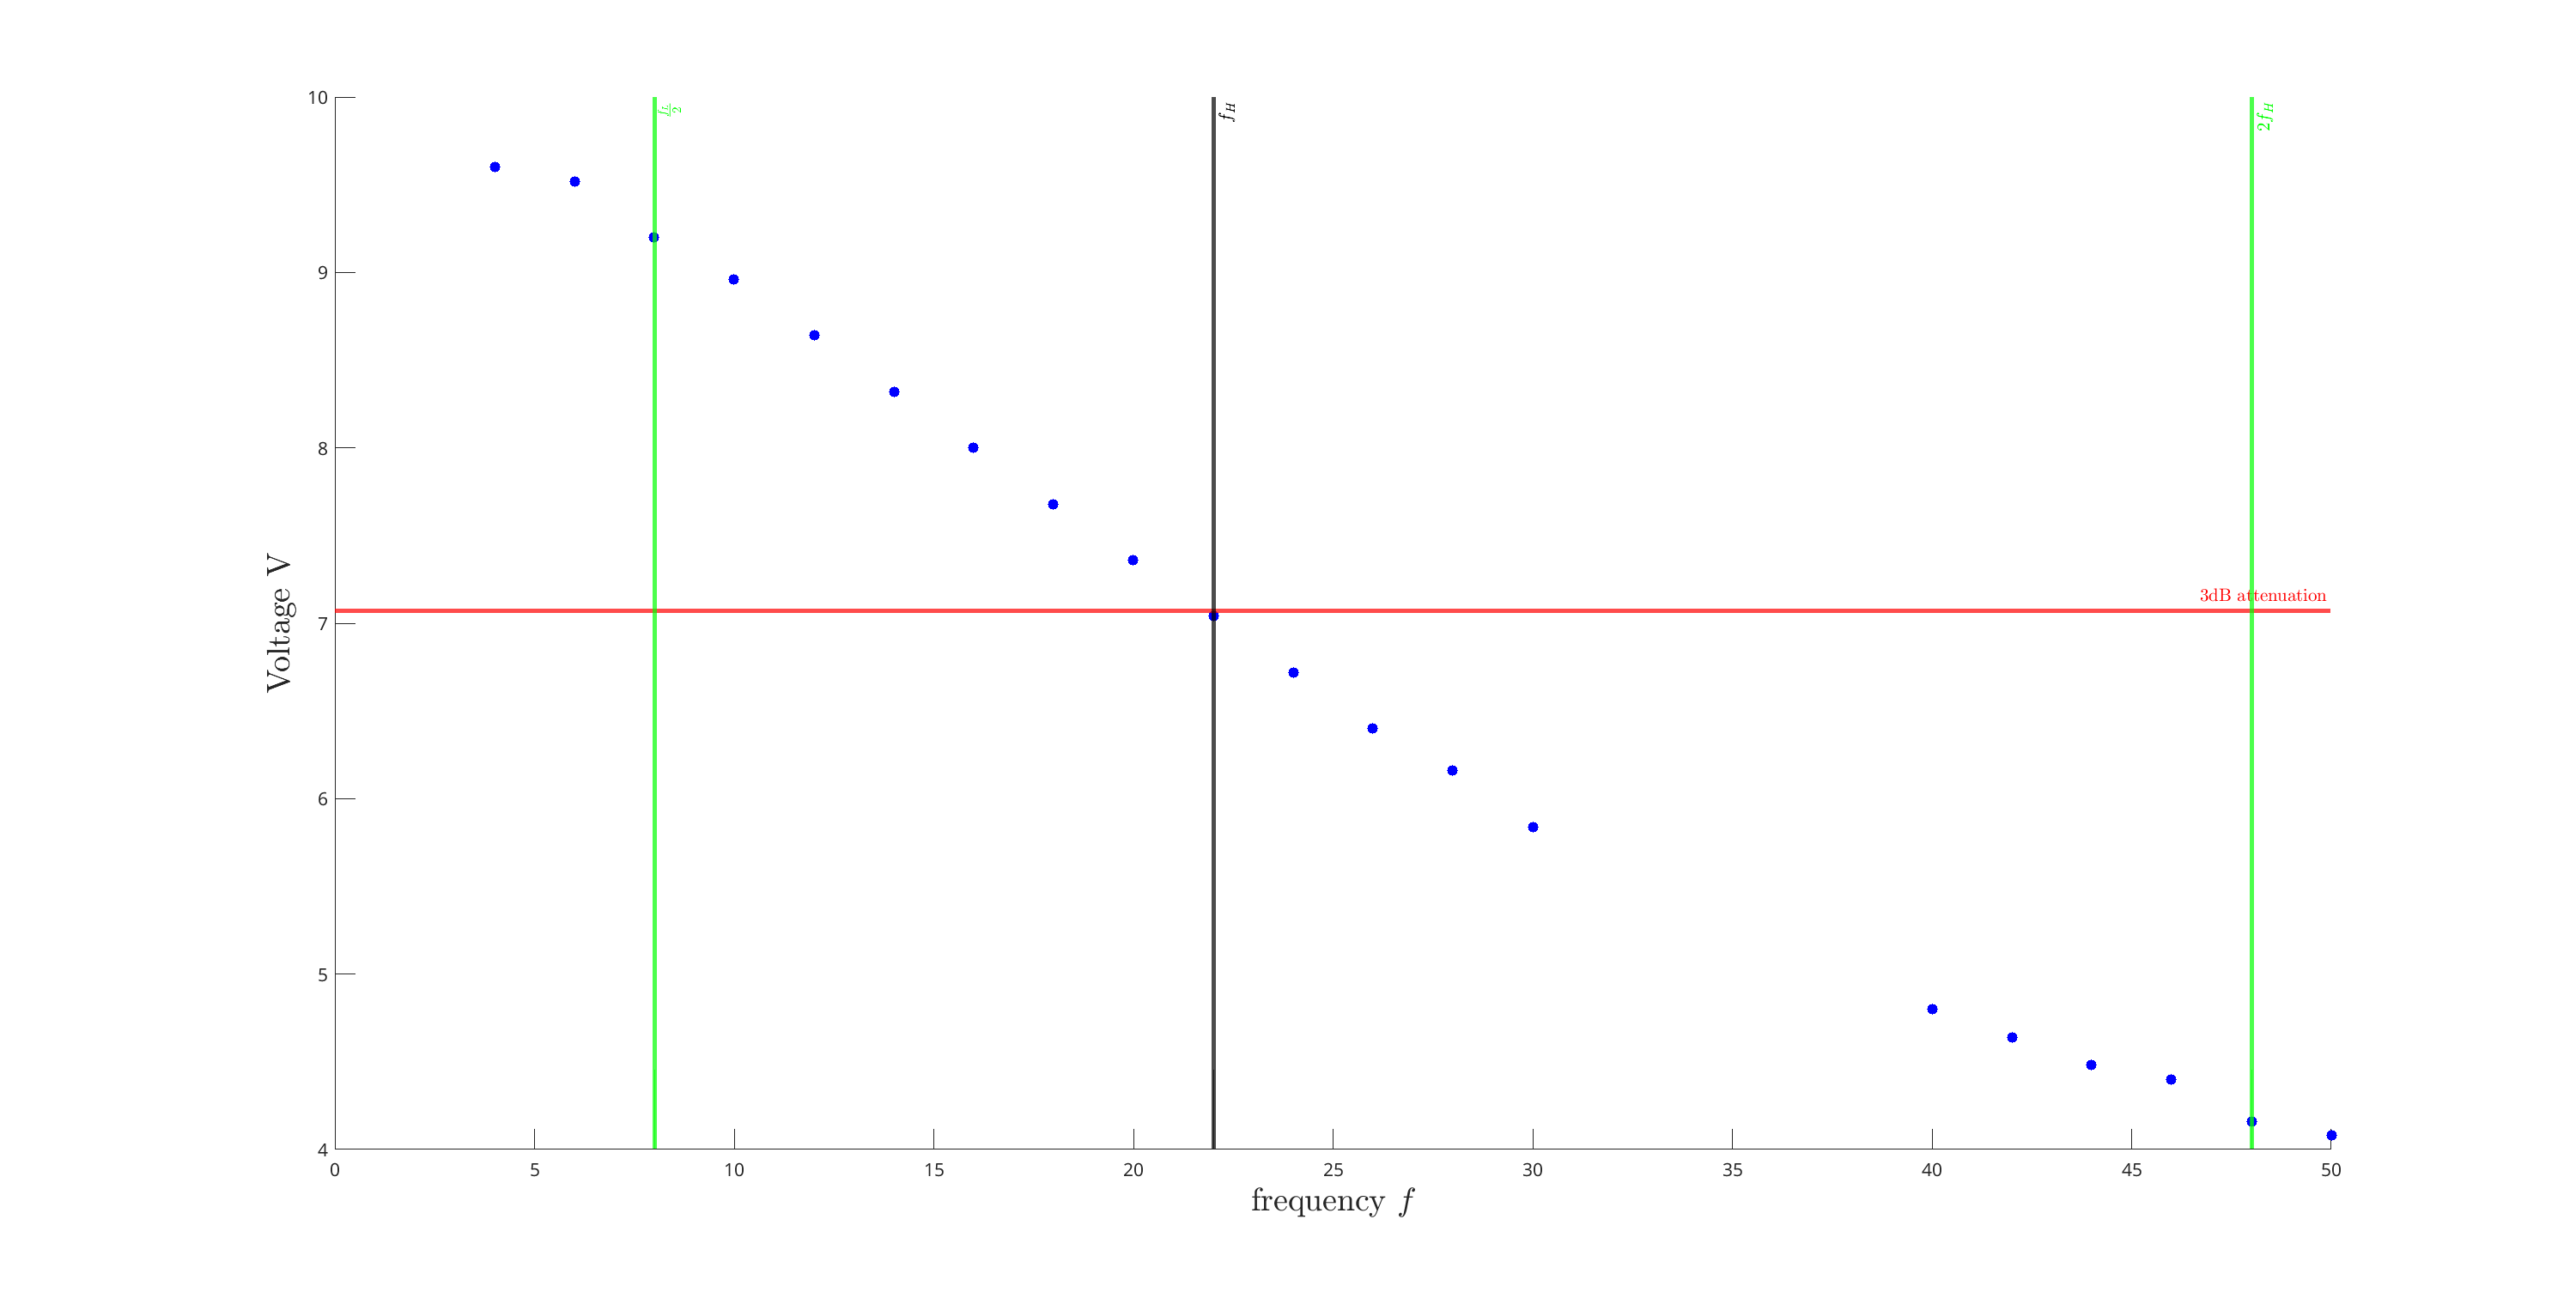
\includegraphics[width=\textwidth]{Active_LPF.png}
  \label{fig:task-2}
\end{figure}


\begin{table}[!ht]
  \centering
  \caption{Frequency response observation table for active low-pass filter with gain 2}
  \begin{tabu}{*[2]{x[c]}}
    \toprule
    \textbf{Signal frequency (kHz)} & \textbf{Output Voltage(V)} \\
    \midrule
      4  & 9.6  \\
      6  & 9.52 \\
      8  & 9.20 \\
      10 & 8.96 \\
      12 & 8.64 \\
      14 & 8.32 \\
      16 & 8.00 \\
      18 & 7.68 \\
      20 & 7.36 \\
      22 & 7.04 \\
      24 & 6.72 \\
      26 & 6.40 \\
      28 & 6.16 \\
      30 & 5.84 \\
      40 & 4.80 \\
      42 & 4.64 \\
      44 & 4.48 \\
      46 & 4.40 \\
      48 & 4.16 \\
      50 & 4.08 \\ 
      \bottomrule
    \end{tabu}
\end{table}

\textbf{Results:}
\begin{enumerate}
  \item The 3dB frequency is 22KHz
  \item The amplitude at $\frac{f_L}{2}=8kHz$ is 9.20V
  \item The amplitude at $2f_H=48kHz$ is 4.16V

\end{enumerate}


\subsection{Task 3}
All signals of frequency 1 kHz, All voltages peak to peak
\begin{enumerate}
  \item $x_1$= 1V, $x_2$ = 1V, $V_{out}$ = 4V
  \item $x_1$= 1V, $x_2$ = 2V, $V_{out}$ = 7V
  \item  $x_1$= 1V, $x_2$ = 3V, $V_{out}$ = 10V
  \item  $x_1$= 2V, $x_2$ = 1V, $V_{out}$ = 5V
  \item  $x_1$= 3V, $x_2$ = 1V, $V_{out}$ = 6V
  \item  $x_1$= 4V, $x_2$ = 1V, $V_{out}$ = 7V
\end{enumerate}
\begin{figure}[!ht]
  \caption{Case 1}
  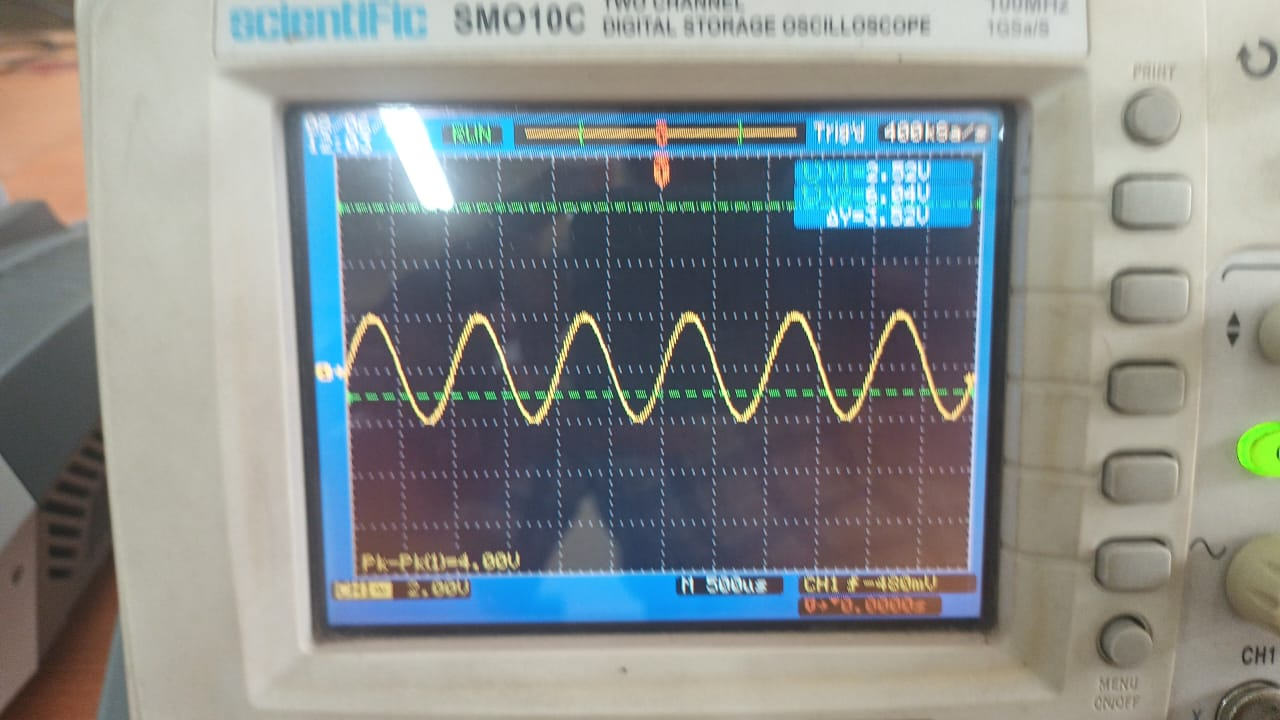
\includegraphics[width=\textwidth]{31.jpeg}
  \label{fig:31}
\end{figure}

\begin{figure}[!ht]
  \caption{Case 2}
  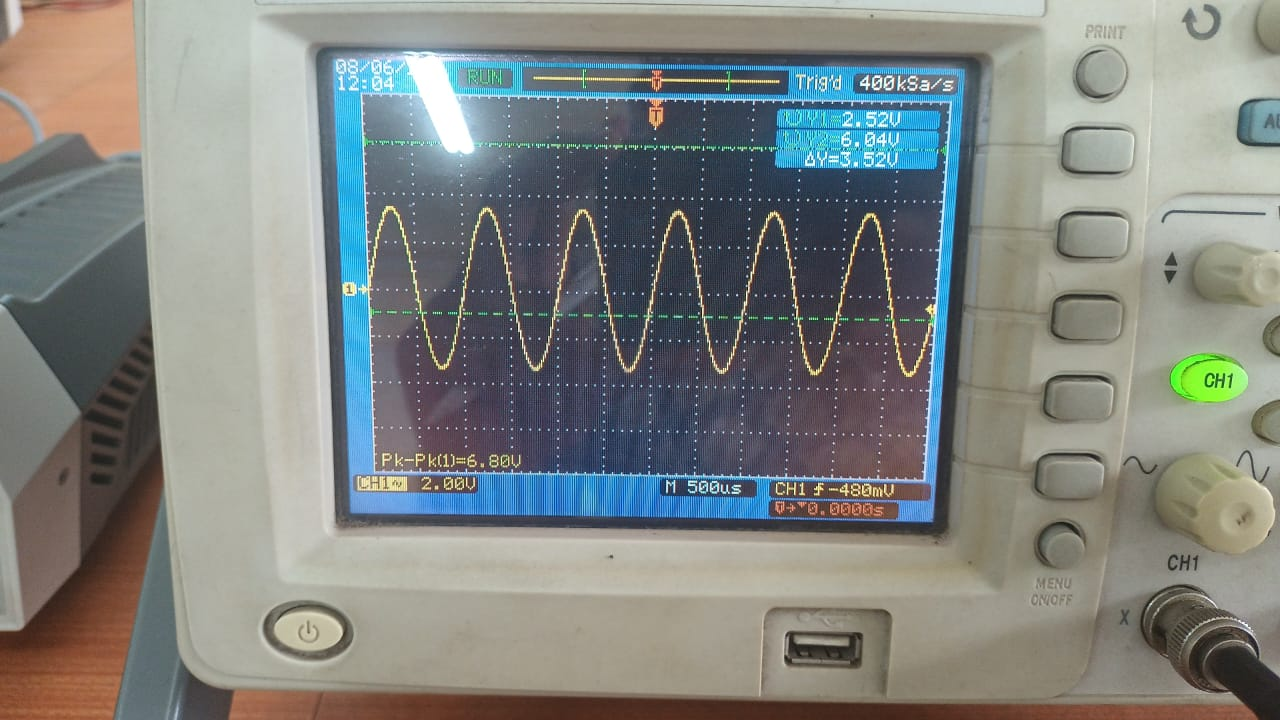
\includegraphics[width=\textwidth]{32.jpeg}
  \label{fig:32}
\end{figure}

\newpage
\begin{figure}[!ht]
  \caption{Case 3}
  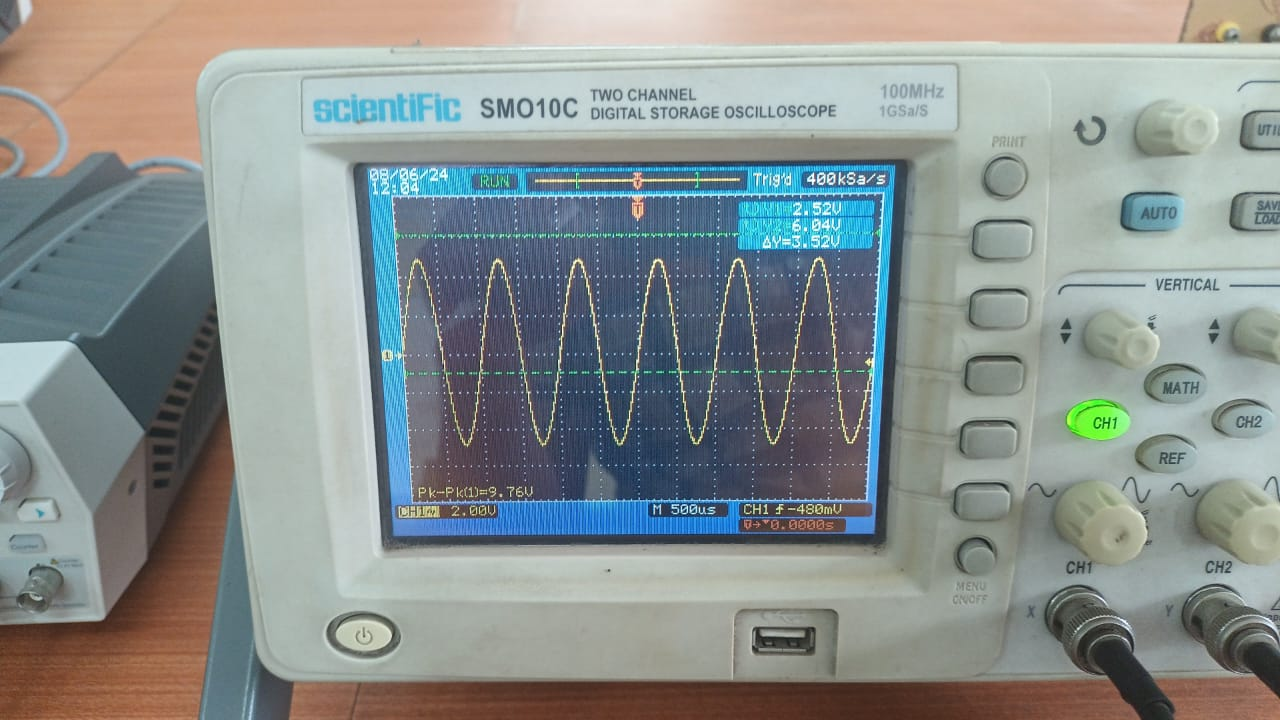
\includegraphics[width=\textwidth]{33.jpeg}
  \label{fig:33}
\end{figure}

\begin{figure}[!ht]
  \caption{Case 4}
  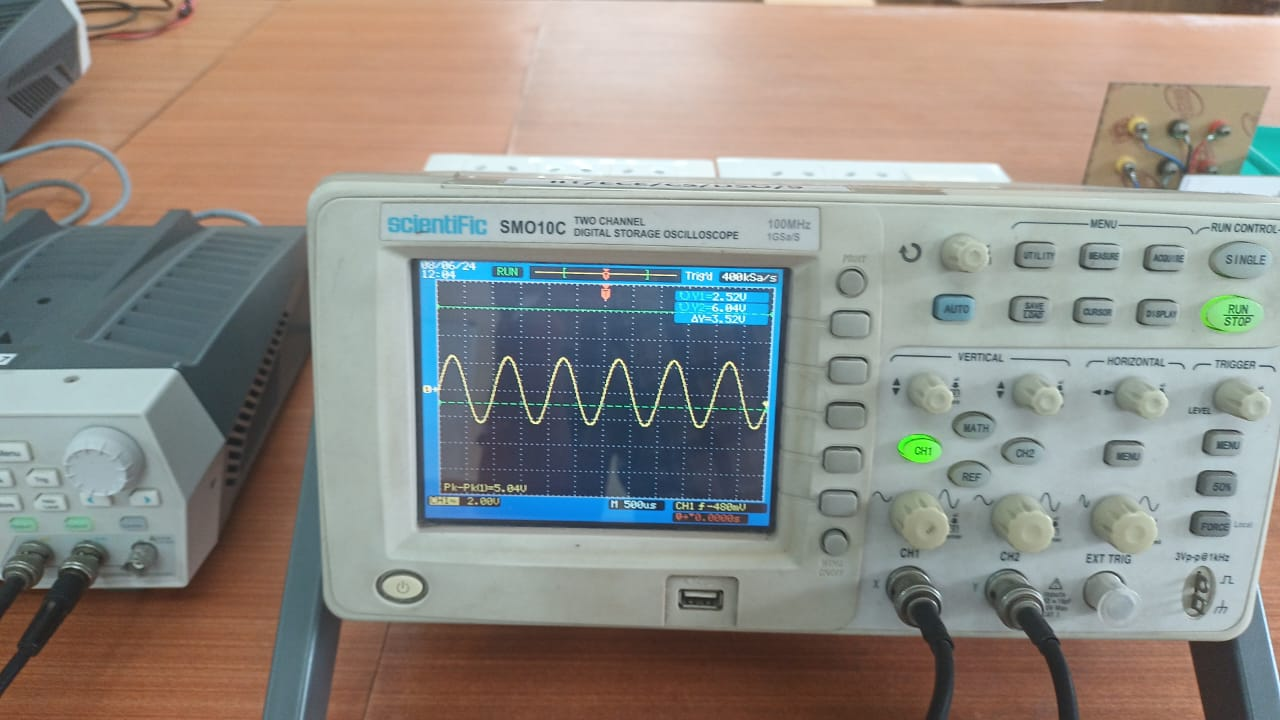
\includegraphics[width=\textwidth]{34.jpeg}
  \label{fig:34}
\end{figure}
\newpage
\begin{figure}[!ht]
  \caption{Case 5}
  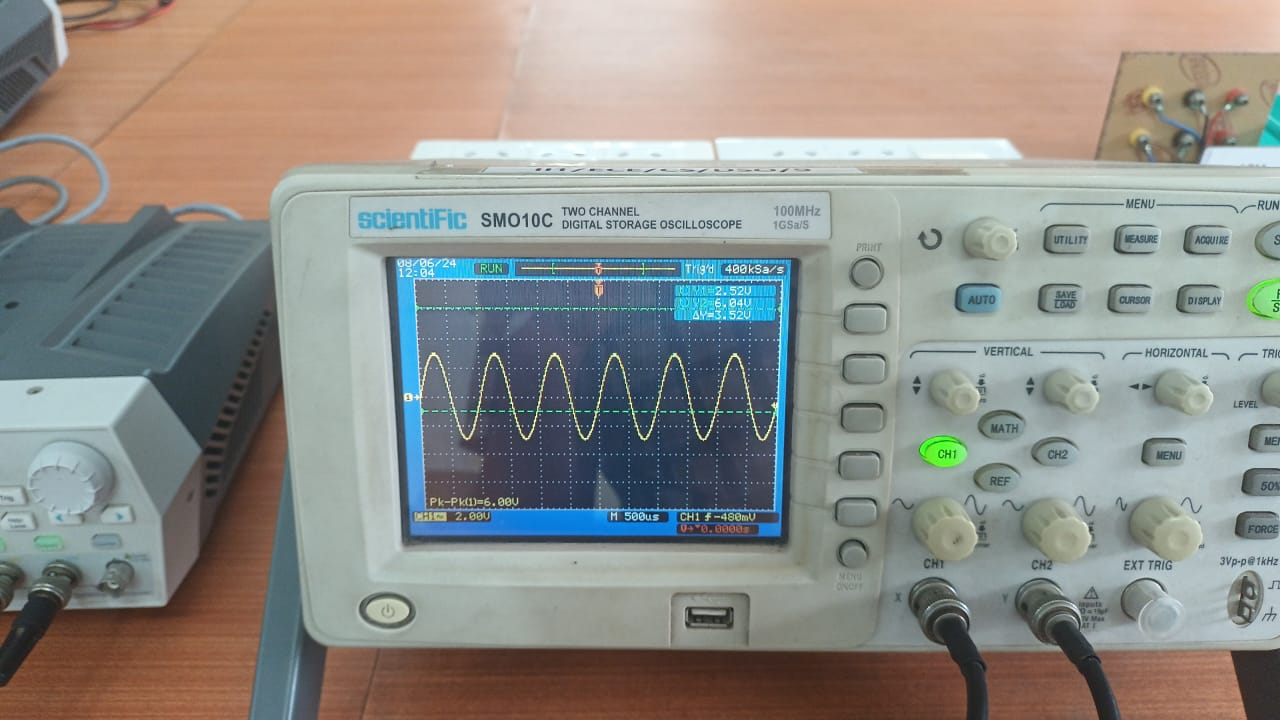
\includegraphics[width=\textwidth]{35.jpeg}
  \label{fig:35}
\end{figure}

\begin{figure}[!ht]
  \caption{Case 6}
  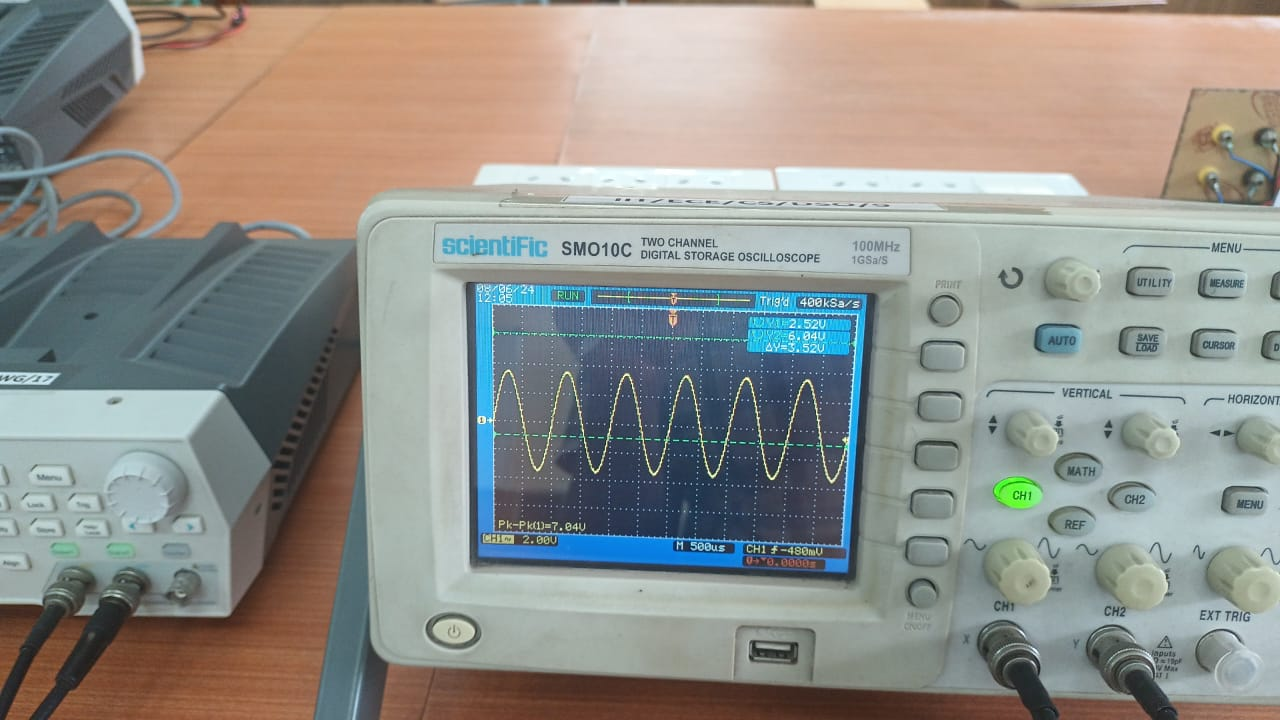
\includegraphics[width=\textwidth]{36.jpeg}
  \label{fig:36}
\end{figure}
\newpage

\vspace{5cm}

\section{Discussion}
\subsection{Samyak Sheersh, 22EC30045}
\begin{enumerate}
  \item We observed that the bandwidth of the band pass filter increased than the expected $f_H-f_L$. We believe this is because the effective resistances seen by the LPF capacitor is increased which leads to $\frac{1}{RC}$ decreasing, which makes $f_L$ go down, and the HPF capacitor sees less resistance which leads to $\frac{1}{RC}$ increasing, which makes $f_H$ go up.
  
  \item We also saw that the active filter gave out a smoother graph, which we think is because the amplification was able to mitigate the loss due to stray resistances and other losses.

  \item Taking the FFT spectrum also showed us that for frequencies within the allowed range, almost all the energy was in a single frequency, the one which we were spending. However for the frequencies which landed outside the acceptable range, the base of the spectrum grew wider. We don't know what the exact mechanism behind this is, and we can't rule out the DSO's precision
\end{enumerate}

\section{Conclusion}
In conclusion, we learned how to design and test the behaviours of passive and active, low-pass, high-pass and band-pass filters.

\end{document}

